\documentclass[times, utf8, seminar, numeric]{fer}
\usepackage{booktabs}
\usepackage{pdfpages}
\usepackage{caption}
\graphicspath{{./prikazi/}}
\bibliographystyle{unsrt}
\usepackage[superscript, biblabel]{cite}
\usepackage{cprotect}
\usepackage{listings}
\lstset{language=,tabsize=4,showstringspaces=false,showtabs=false,breaklines=true,breakatwhitespace=true,basicstyle=\ttfamily,frame=single}

\begin{document}

\title{Obrada audio signala u stvarnom vremenu}

\author{Fran Jelavić}

\voditelj{Ivan Đurek}
\maketitle

\tableofcontents

\chapter{Uvod}

Obrada audio signala u stvarnom vremenu je neophodna u mnogim primjenama kao što je kompresija i prijenos audio informacija, poništavanje buke i uklanjanje šuma, prepoznavanje glasa te obrada i produkcija glazbe. Cilj ovog seminara pružiti je pregled temeljnih koncepata digitalne obrade signala i digitalnog zvuka, te demonstrirati kako implementirati pojedine audio efekte u stvarnom vremenu koristeći Python programski jezik.

U seminaru se prvenstveno uvode osnovni koncepti DSP-a, uključujući svojstva digitalnih signala, uzorkovanje, kvantizaciju i brzu Fourierovu transformaciju. Glavni fokus seminara usredotočen je na audio efekte, specifičnije o tome kako rade efekti reverb, delay i chorus. Dodatno, seminar se dotiče jednostavne implementacije algoritama za navedene efekte u programskom jeziku Python te se raspravlja o njihovoj optimizaciji.

Cilj ovog seminara je omogućiti razumijevanje principa i implementacije pojedinih algoritma kao primjera osnovnih koncepta obrade audio signala u stvarnom vremenu.


\chapter{Osnovni koncepti DSP-a}

Digitalni signal niz je brojeva koji predstavljaju amplitudu signala kroz kontinuirano vrijeme uzorkovano u pravilnim intervalima. Proces uzorkovanja signala u kontinuiranom vremenu uključuje mjerenje njegove amplitude u određenim vremenskim pomacima i pretvaranje tih mjerenja u diskretni niz brojeva (nula i jedinica).\cite{dueck2005digital}

\section{Kvantizacija}

Koncept kvantizacije uključuje mapiranje kontinuiranih vrijednosti amplitude u konačni skup diskretnih razina amplitude. Budući da računala mogu prikazati samo signale s konačnim brojem bitova, kvantizacija je bitna kako bi se zaobišao problem nedostatka beskonačne memorije za pohranu signala.\cite{tsividis2004digital}

Proces kvantizacije podrazumijeva dijeljenje kontinuiranog raspona vrijednosti amplituda na konačan broj razina i preslikavanje svake od tih vrijednosti na najbližu razinu. Broj razina određen je brojem bitova koji se koriste za predstavljanje signala. Na primjer, signal predstavljen sa 16 bitova može imati 2$^{16}$ (65,536) različitih razina amplitude.

Kvantizacija uzrokuje određenu količinu greške, poznata kao šum kvantizacije, koja se ističe kao razlika između izvorne kontinuirane vrijednosti amplitude i njene kvantizirane vrijednosti. Povećanjem broja bitova koji se koriste za kvantizaciju ublažit će se šum kvantizacije, a time će obrađeni signal biti kvalitetniji i točniji svojem izvornom signalu. Bitno je napomenuti da povećanje broja bitova signala usporava sam proces obrade signala te je memorijski zahtjevnije.

U praksi je kvantizacija vrlo bitan korak pri početku obrade signala, budući da utječe na kvalitetu signala. Pogreške pri kvantizaciji uzrokovat će pogreške u daljnjoj obradi poput izobličenja, šuma i drugih artefakata. U kontekstu audio signala, to može rezultirati u nepoželjnom i "nečistom" zvuku koji narušava kvalitetu zvučnog zapisa. Iz tih razloga, bitno je prije samog početka obrade signala odrediti odgovarajući broj bitova za kvantizaciju koji omogućiti kvalitetnu, ali i brzu obradu signala.\cite{gersho2012vector}

\section{FFT}

Brza Fourierova transformacija (eng. \textit{Fast Fourier Transform} - FFT) učinkovit je algoritam za računanje diskretne Fourierove transformacije (eng. \textit{Discrete Fourier Transform} - DFT), matematičkog alata koji se koristi za pretvaranje digitalnog signala u njegovu reprezentaciju u frekvencijskoj domeni. Drugim riječima, pretvara digitalni signal u skup brojeva pomoću kojeg se da raspoznati najzastupljenije frekvencije u signalu. FFT je posebno koristan za analizu audio signala u frekvencijskoj domeni, što omogućuje manipulaciju audio signalom mijenjajući njegov frekvencijski sadržaj.\cite{heideman1985gauss}

\subsection{Način rada FFT-a}

Obradom signala pomoću FFT-a, na izlazu se dobiva slijed brojeva u nizu koji predstavlja domenu frekvencija obrađenog signala, npr.:
\begin{verbatim}
	fft_output_array = [23, 43, 65, 443, 321, 54, 56 ...]
\end{verbatim}
Svaki indeks ovog niza naziva se \textit{bin} te predstavlja određen raspon frekvencija. Broj na svakom indeksu je intenzitet frekvencija u rasponu koji predstavlja. Što je broj veći, to je veća zastupljenost frekvencija unutar svoga raspona. Raspon frekvencija u pri svakom indeksu ovisi o rezoluciji (eng. \textit{resolution}) koja se može izraziti na sljedeći način:
\begin{verbatim}
	resolution = sampling_rate / fft_size
\end{verbatim}
pri čemu je \verb|fft_size| veličina spremnika za uzorke (eng. \textit{buffer size}).\cite{lourde2009digital} Veličina \textit{buffer}-a povezana je s vremenom koje je potrebno za obradu signala, pri čemu manje veličine stvaraju manje kašnjenje, ali predstavljaju veći teret pri procesiranju i veću mogućnost grešaka.\cite{focusrite_2022}

Kako bi se raspoznale frekvencije po \textit{bin}-ovima, može se koristiti sljedeća formula:
\begin{verbatim}
	start_frequency = bin_number * resolution
\end{verbatim}
pri čemu je \verb|start_frequency| početna frekvencija raspona.\cite{gustine_2021} Raspon frekvencija bi time bio od \verb|start_frequency| do \verb|start_frequency + resolution|.

\section{Konvolucija}

Konvolucija temeljna je operacija u digitalnoj obradi signala koja se koristi za filtriranje i implementaciju audio efekata kao što su \textit{reverb} i kašnjenje (eng. \textit{delay}). Konvolucija se odnosi na množenje dvaju signala i integriranje rezultata kroz vrijeme.\cite{krishna2017digital} 

U kontinuiranom signalu, jednadžba konvolucije izvornog signala s impulsnim odzivom izražava se kao:
\begin{equation*}
	y(t) = \int_{-\infty}^{\infty} x(t) \cdot h(t - \tau) \,d\tau
\end{equation*}
gdje $y(t)$ predstavlja visinu amplitude rezultatnog signala u određenoj jedinici vremena $t$. Visina amplitude izvornog signala predstavljena je varijablom $x(t)$, dok $h(t)$ predstavlja visinu amplitude impulsnog odziva. Izraz $h(t - \tau)$ predstavlja visinu amplitude impulsnog odziva u trenutku $t - \tau$, gdje $\tau$ označava početak impulsnog odziva u vremenskoj domeni $t$. Jednadžba predstavlja kontinuiranu sumu (izraženu integralom) umnoška amplituda izvornog signala i impulsnog odziva kroz vremensku domenu.

U audio obradi se konvolucija koristi kako bi se simuliralo okruženje koje mijenja zvuk. Na primjer, reverberacija se može simulirati konvolucijom audio signala s impulsnim odzivom kako bi se predstavila refleksija zvuka u prostoriji.

Implementaciju konvolucije moguće je postići FFT-om. Konvolucija se na taj način postiže množenjem frekvencijskih domena signala i vraćanjem rezultata u vremensku domenu korištenjem inverzne Fourierove transformacije (eng. \textit{Inverse Fourier Transform} - IFT).

U praksi konvolucija zna biti računalno zahtjevna, posebice za duže audio signale. Stoga se mogu primjeniti razni optimizacijski postupci za smanjenje složenosti konvolucije, npr. korištenje manje veličine spremnika za uzorke pri FFT-u (eng. \textit{buffer size}).\cite{krishna2017digital}


\chapter{Audio efekti}

\section{Delay}

Kašnjenje (eng. \textit{delay}) je audio efekt koji stvara dojam ponavljanja zvuka ili jeke. To se postiže reprodukcijom odgođene verzije izvornog audio signala. U svom najjednostavnijem obliku, kašnjenje uključuje reprodukciju kopije izvornog audio signala nakon određenog vremena. Ovo stvara ponovljeni zvuk koji se čuje nakon izvornog zvuka. Količina vremena između izvornog zvuka i odgođenog zvuka poznata je kao vrijeme kašnjenja (eng. \textit{delay time}) i obično se mjeri u milisekundama (ms).\cite{zolzer2022digital}

Odgođeni signal može se modificirati za stvaranje različitih vrsta efekata kašnjenja, kao što su \textit{flanger} i \textit{chorus} koji nastaju modulacijom vremena kašnjenja tijekom vremena.
U \textit{flanger}-u modulacijom vremena kašnjenja stvara se efekt poput zvuka kroz PVC cijevi.  U \textit{chorus}-u modulacijom vremena kašnjenja stvara se efekt koji simulira zvuk od više glasova ili instrumenata koji sviraju istu ulogu.\cite{dattorro1997effect}

Kašnjenje se može koristiti za stvaranje različitih efekata. Na primjer, kratka vremena kašnjenja (manje od 30 ms) mogu se koristiti za stvaranje osjećaja prostora i dubine zvuka, dok duža vremena odgode mogu stvoriti izraženiji efekt jeke.

\section{Reverb}

Reverberacija ili odjek (eng. \textit{reverberation} ili kraće \textit{reverb}) audio je efekt koji simulira akustične karakteristike prostora, kao što je soba ili koncertna dvorana, dodavanjem refleksije i slabljenja audio signalu. Time se u zvukom postiže osjećaj uronjenosti u virtualnom okruženju. Osnovna ideja reverberacije je simulacija načina na koji se zvučni valovi odbijaju od površina u prostoru i slabe tijekom vremena. To se postiže konvolviranjem audio signala s impulsnim odzivom koji predstavlja refleksiju i slabljenje zvuka u određenom prostoru.\cite{lloyd1937music}

Impulsni odziv (eng. \textit{impulse response}) dobiva se puštanjem kratkog praska zvuka u prostoru i snimanjem rezultirajućeg zvuka kako se smanjuje tijekom vremena. Rezultirajući valni oblik uključuje refleksiju zvuka od površina u prostoru, kao i slabljenje zvuka radi površinske apsorpcije i raspršenja tijekom vremena. Kada se audio signal konvolvira s impulsnim odzivom, rezultirajući signal se modificira tako da uključuje refleksije i slabljenje zvuka u simuliranom prostoru. Što je dulji odziv impulsa, to će više refleksija i slabljenja biti dodano signalu, stvarajući izraženiji osjećaj prostora.\cite{gardner2002reverberation}

Postoji mnogo različitih vrsta \textit{reverb}-a, od kojih svaka ima svoje jedinstvene karakteristike. Neki uobičajeni tipovi reverbiranja uključuju sobni (eng. \textit{room}), dvoranski (eng. \textit{hall}), pločasti (eng. \textit{plate}) i opružni (eng. \textit{spring}) \textit{reverb}. Svaka vrsta reverberacije simulira drugu vrstu prostora i ima svoj poseban zvuk.

Najbitniji parametri za \text{reverb} uključuju slabljenje (eng. \textit{decay}), veličina (virtualnog) prostora, pred-kašnjenje (eng. \textit{pre-delay}), difuzija (eng. \textit{diffusion}) i prigušivanje (eng. \textit{damping}).\cite{nativeinstrumentsReverbEssential} U svrhu ovog seminara, za implementaciju jednostavnog \textit{reverb}-a dovoljno će biti proći \textit{decay}.

\subsection{Decay}
Vrijeme slabljenja (eng. \textit{decay time}), poznato i kao vrijeme odjeka (eng. \textit{reverb time}) je vrijeme koje je potrebno zvuku da prestane odjekivati. Drugim riječima, vrijeme slabljenja je koliko dugo traje titranje zvuka u prostoru od kad je titranje izvora zvuka prestalo.\cite{nativeinstrumentsReverbEssential}
Kod reverberacije, vrijeme slabljenja obično se kontrolira podešavanjem brzine kojom zvučnu energiju apsorbiraju površine u virtualnom prostoru. Ova stopa apsorpcije često se modelira korištenjem eksponencijalne funkcije slabljenja, gdje je vrijeme slabljenja vrijeme koje je potrebno da se zvučna energija smanji za 60 decibela (dB) ili jednu tisućinku svoje izvorne vrijednosti:
\begin{equation*}
	slabljenje = e^{-\frac{1}{f_s * \tau}}
\end{equation*}
Frekvencija uzorkovanja (eng. \textit{sampling frequency}) predstavljena je $f_s$, dok $\tau$ predstavlja vrijeme slabljenja.

\section{Chorus}

Refren (eng. \textit{chorus}) je popularan audio efekt koji se često koristi u glazbenoj produkciji i obradi audio signala. Stvoren je pomoću efekta kašnjenja s moduliranim vremenom kašnjenja, koji simulira zvuk više glasova ili instrumenata koji sviraju istu ulogu.\cite{dattorro1997effect}

Vrijeme kašnjenja u \textit{chorus}-u modulira se niskofrekventnim oscilatorom (eng. \textit{Low-frequency Oscilator} - LFO), koji stvara raštimirani efekt koji ostavlja dojam da više izvora svira zajedno. Učinak raštimiranja (eng. \textit{detuning}) može se prilagoditi kako bi se stvorile različite razine dubine modulacije, a brzina LFO-a može se prilagoditi kako bi se stvorile različite brzine modulacije.

\textit{Chorus} se može koristiti na različite načine za poboljšanje zvuka ili glazbenog miksa. Na primjer, može se koristiti za stvaranje osjećaja dubine i prostora, za davanje dubine glavnom vokalu ili davanje težine gitari pri refrenu pjesme. Također se može koristiti za stvaranje zanimljivih i neobičnih efekata, kao što su podvodni ili nezemaljski zvukovi.

\pagebreak
\section{Vizualizacija}
\subsection{Delay}
\begin{figure}[!htb]
	\centerline{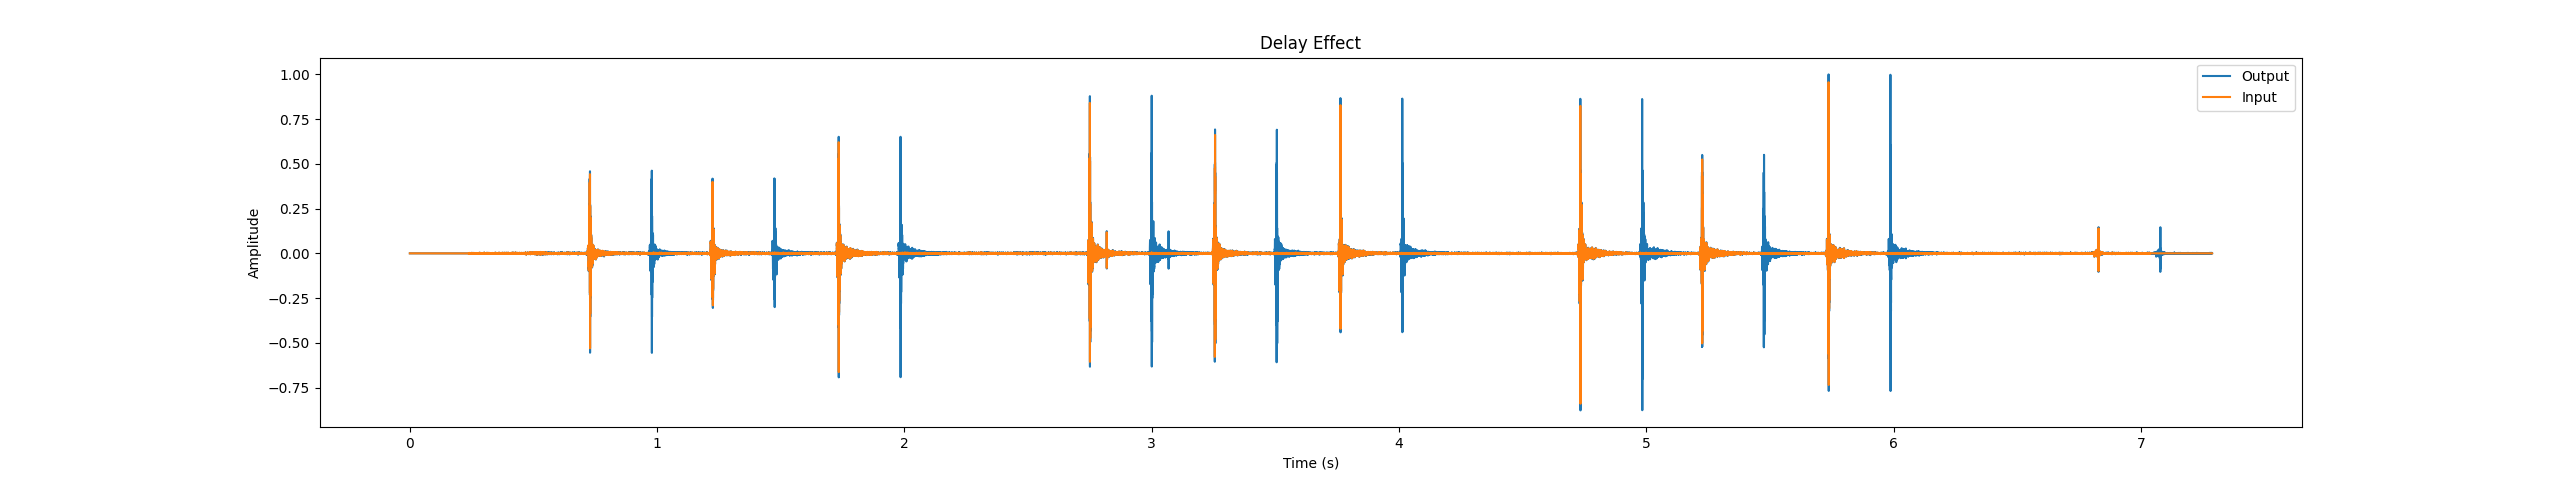
\includegraphics[width=1.75\textwidth]{delay_finger-snapping.png}}
	\caption{\textit{Delay}: pucketanje prstima}
	\label{fig}
\end{figure}
\begin{figure}[!htb]
	\centerline{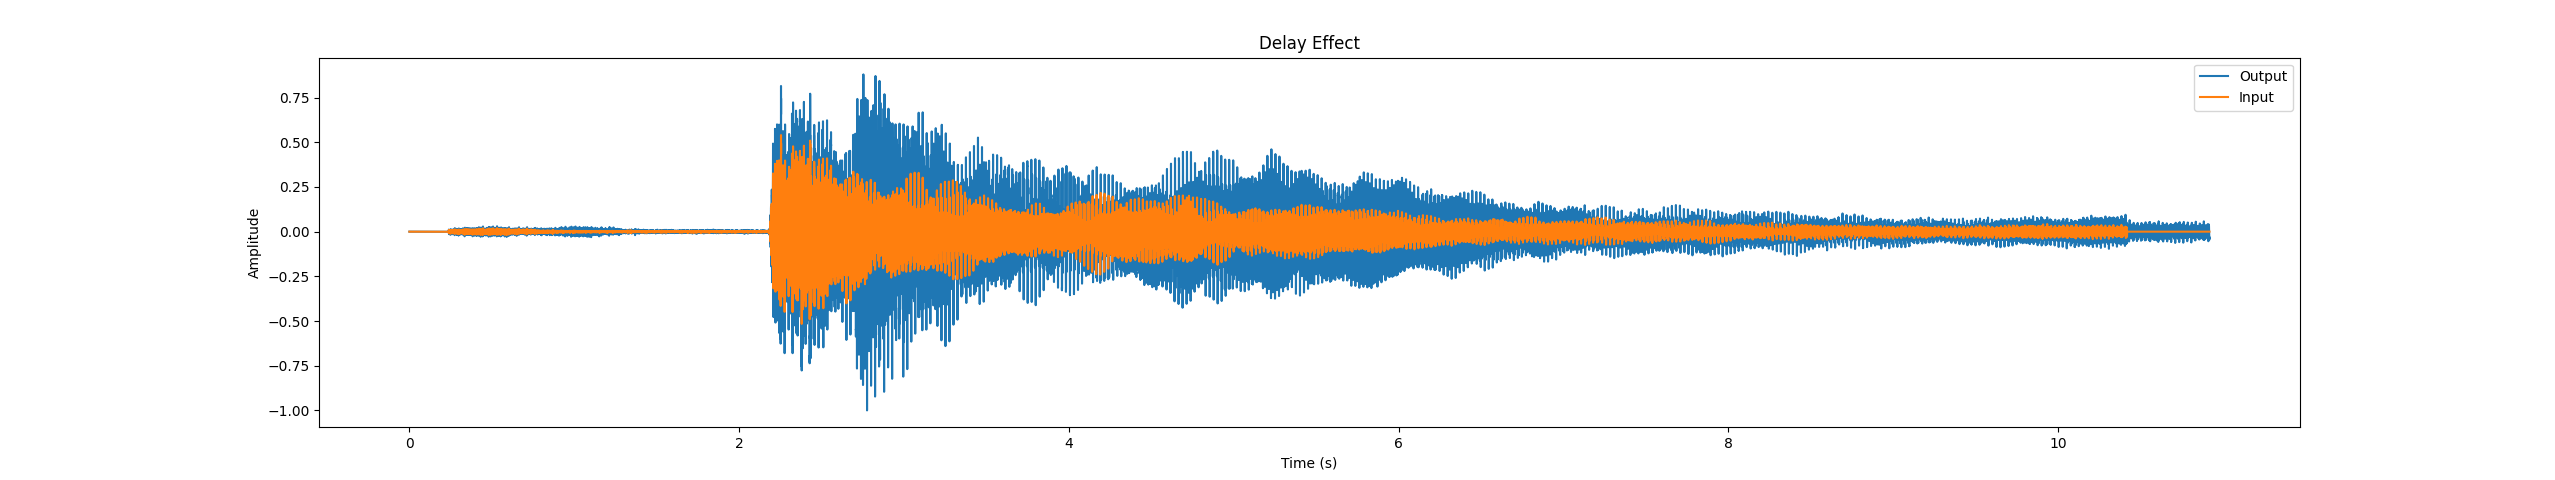
\includegraphics[width=1.75\textwidth]{delay_strum.png}}
	\caption{\textit{Delay}: prolaz (eng. \textit{strum}) po žicama gitare}
	\label{fig}
\end{figure}
\begin{figure}[!htb]
	\centerline{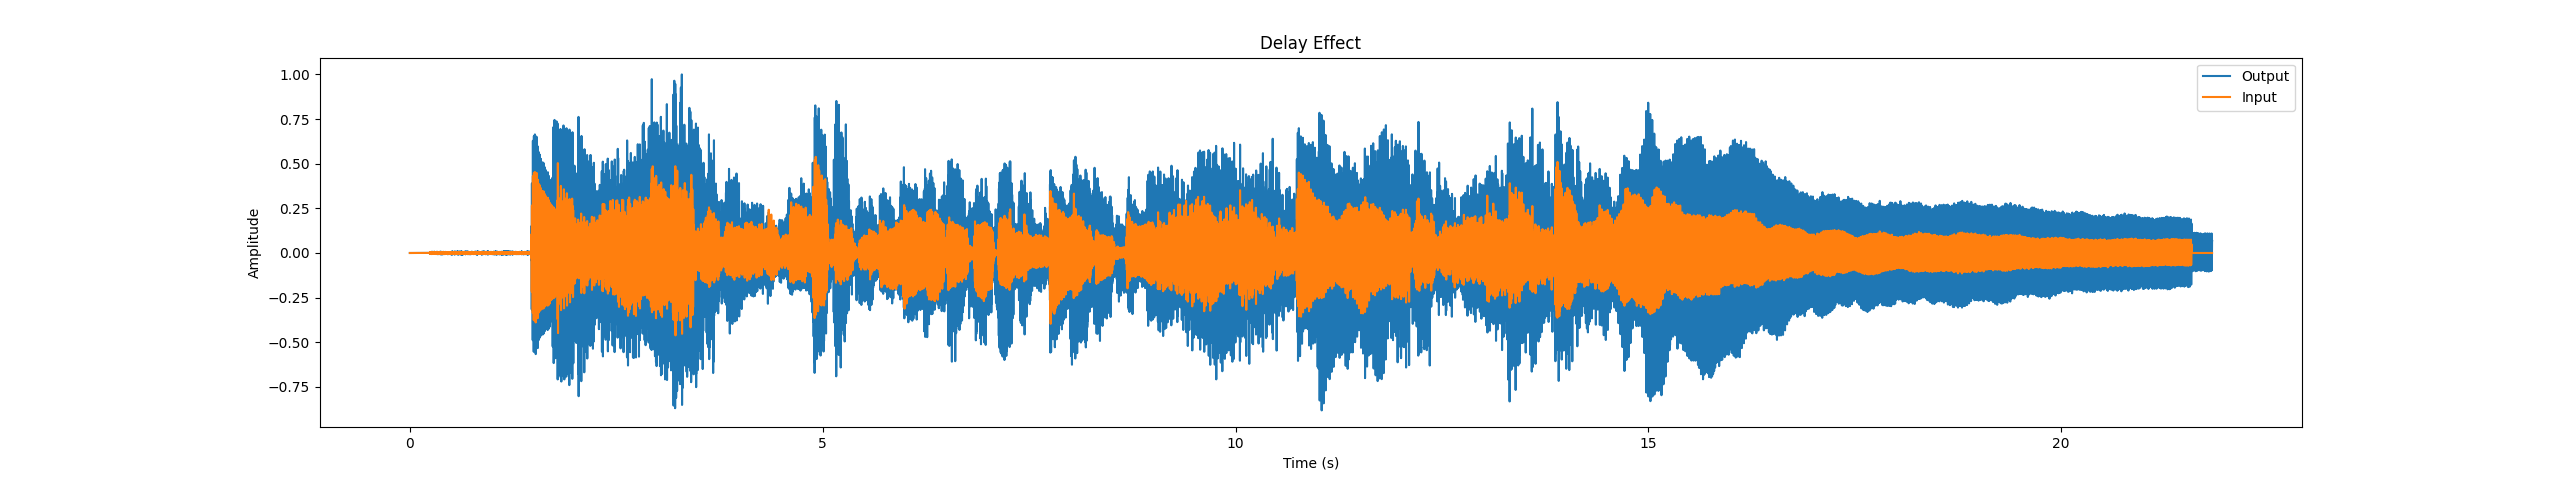
\includegraphics[width=1.75\textwidth]{delay_rising-sun.png}}
	\caption{\textit{Delay}: rif (eng. \textit{riff}) pjesme \textit{House of the Rising Sun}}
	\label{fig}
\end{figure}

\pagebreak
\subsection{Reverb}
\begin{figure}[!htb]
	\centerline{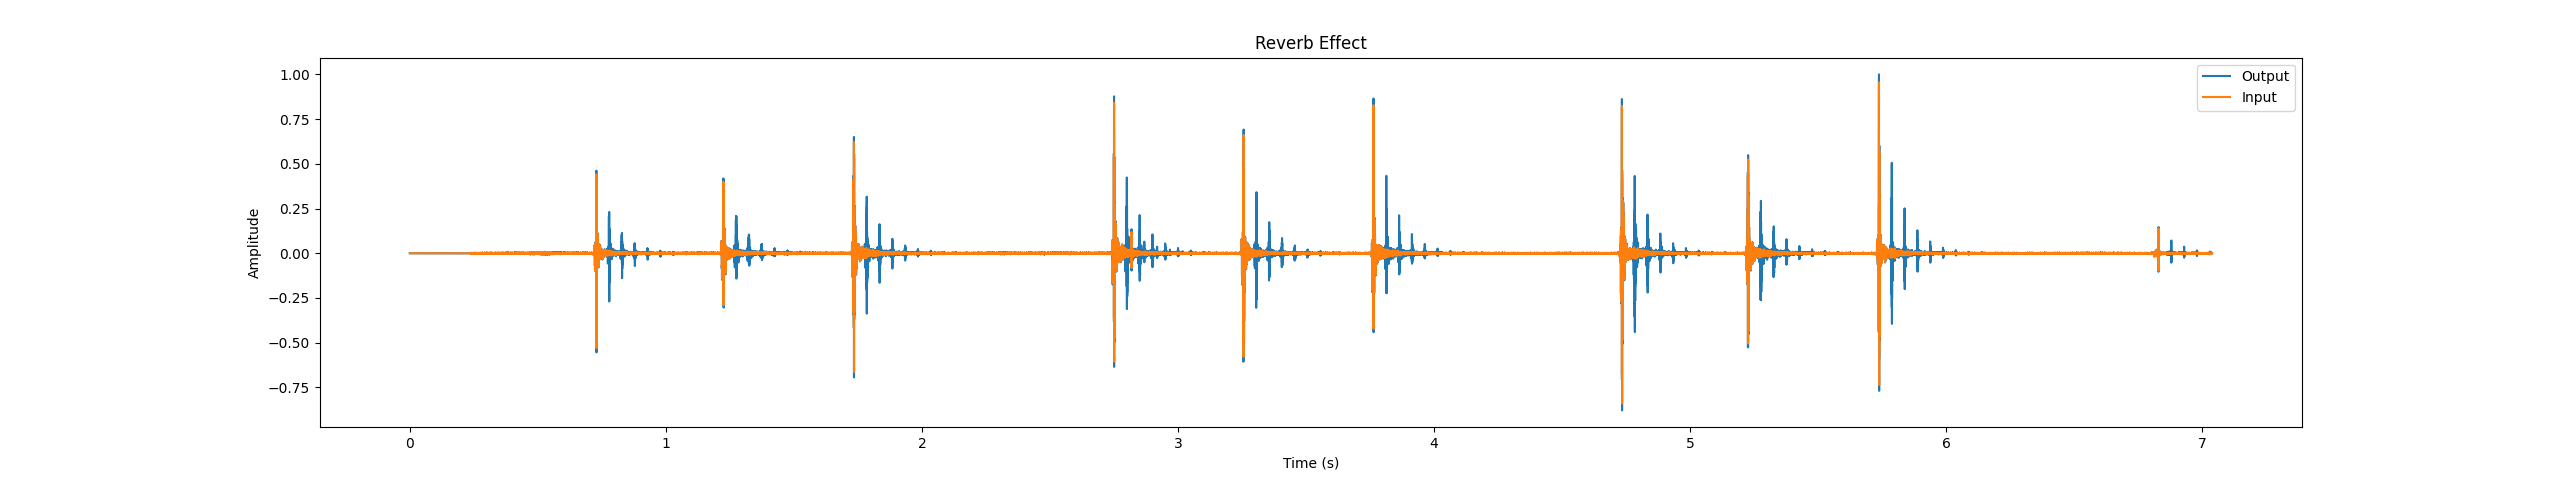
\includegraphics[width=1.75\textwidth]{reverb_finger-snapping.png}}
	\caption{\textit{Reverb}: pucketanje prstima}
	\label{fig}
\end{figure}
\begin{figure}[!htb]
	\centerline{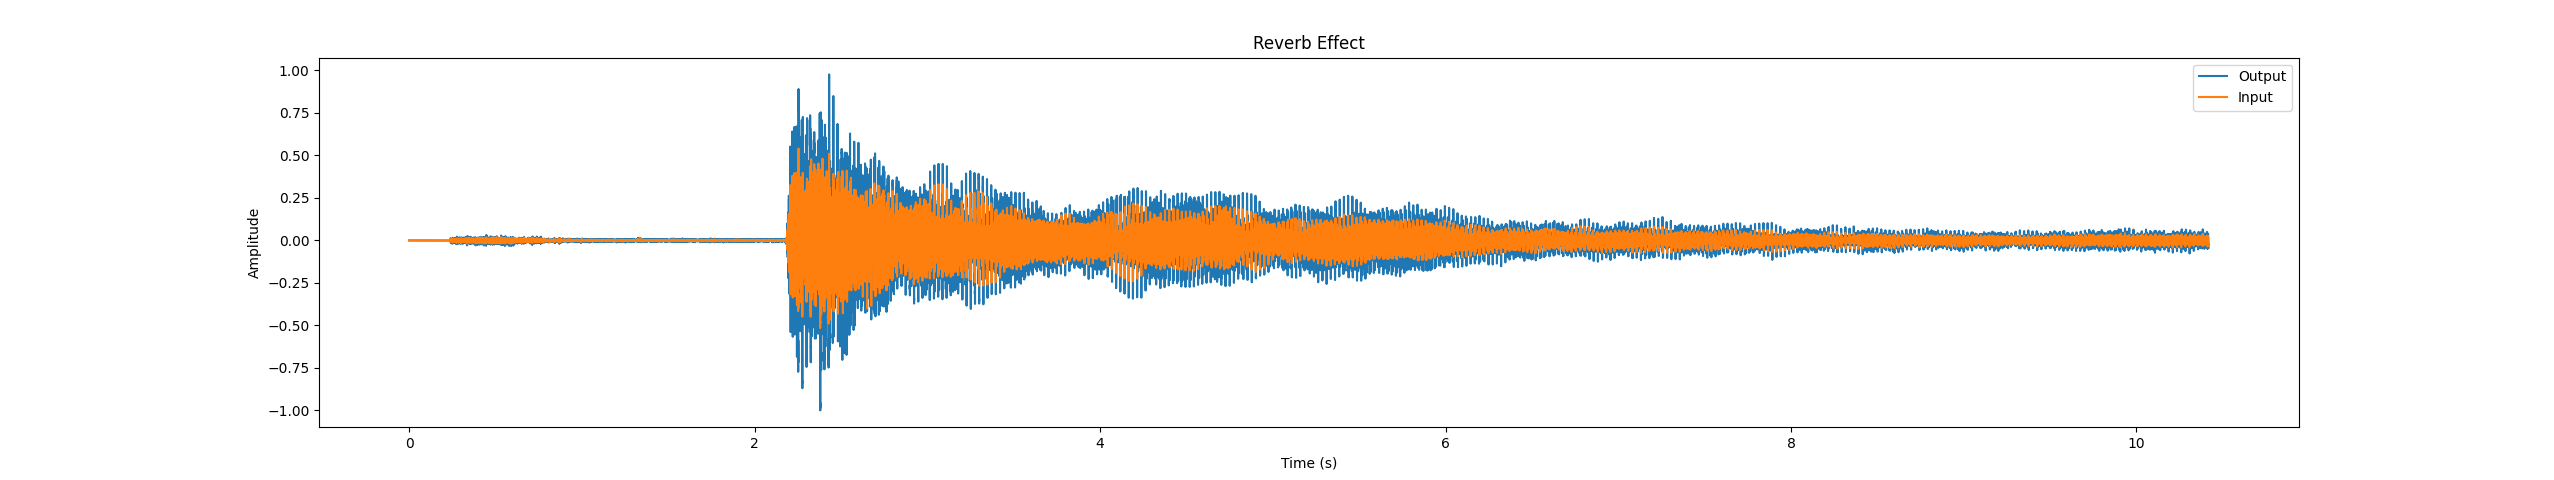
\includegraphics[width=1.75\textwidth]{reverb_strum.png}}
	\caption{\textit{Reverb}: prolaz (eng. \textit{strum}) po žicama gitare}
	\label{fig}
\end{figure}
\begin{figure}[!htb]
	\centerline{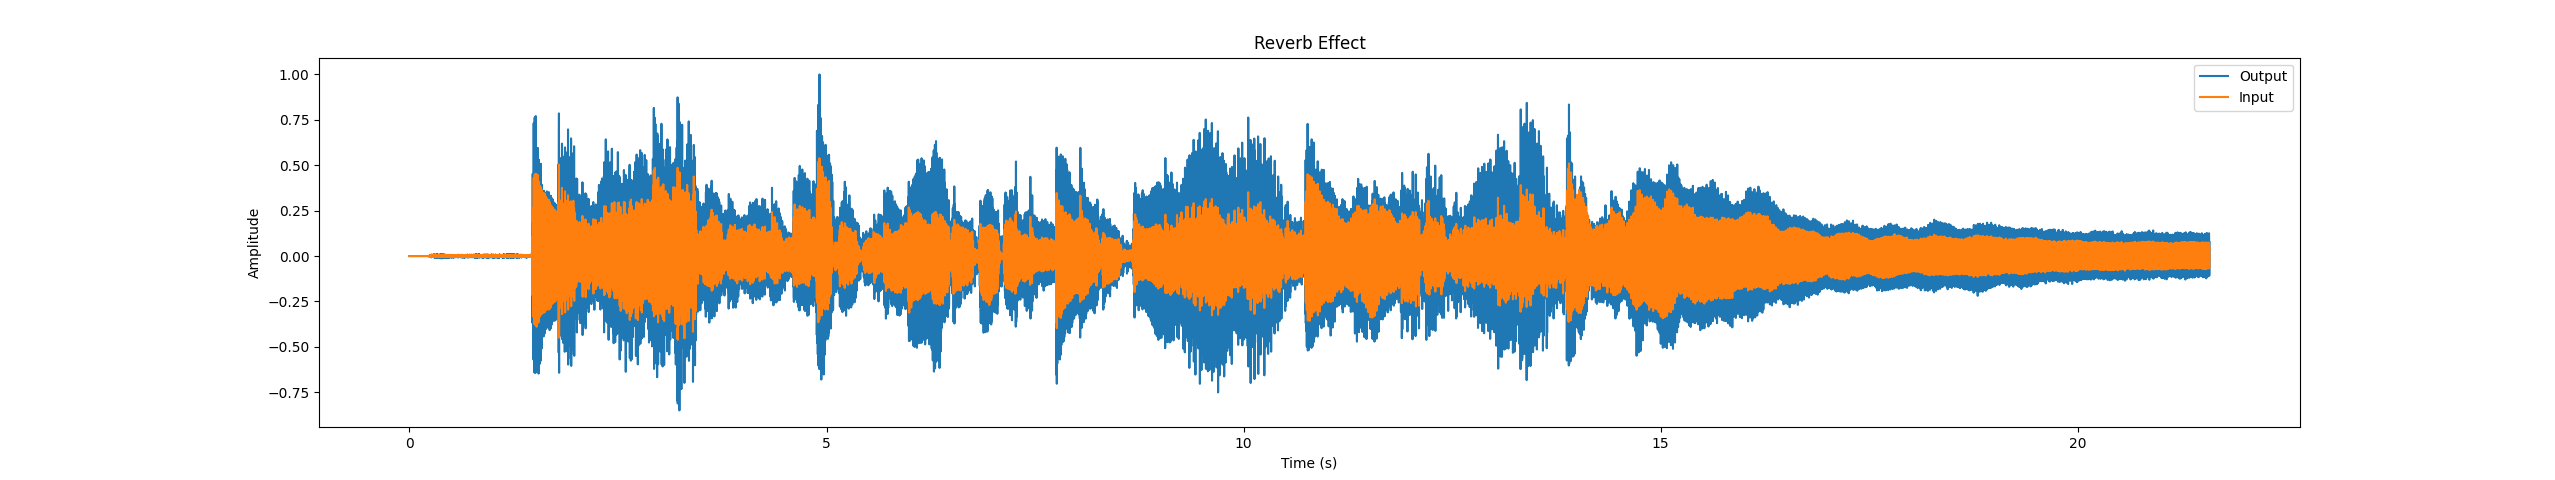
\includegraphics[width=1.75\textwidth]{reverb_rising-sun.png}}
	\caption{\textit{Reverb}: rif (eng. \textit{riff}) pjesme \textit{House of the Rising Sun}}
	\label{fig}
\end{figure}

\pagebreak
\subsection{Chorus}
\begin{figure}[!htb]
	\centerline{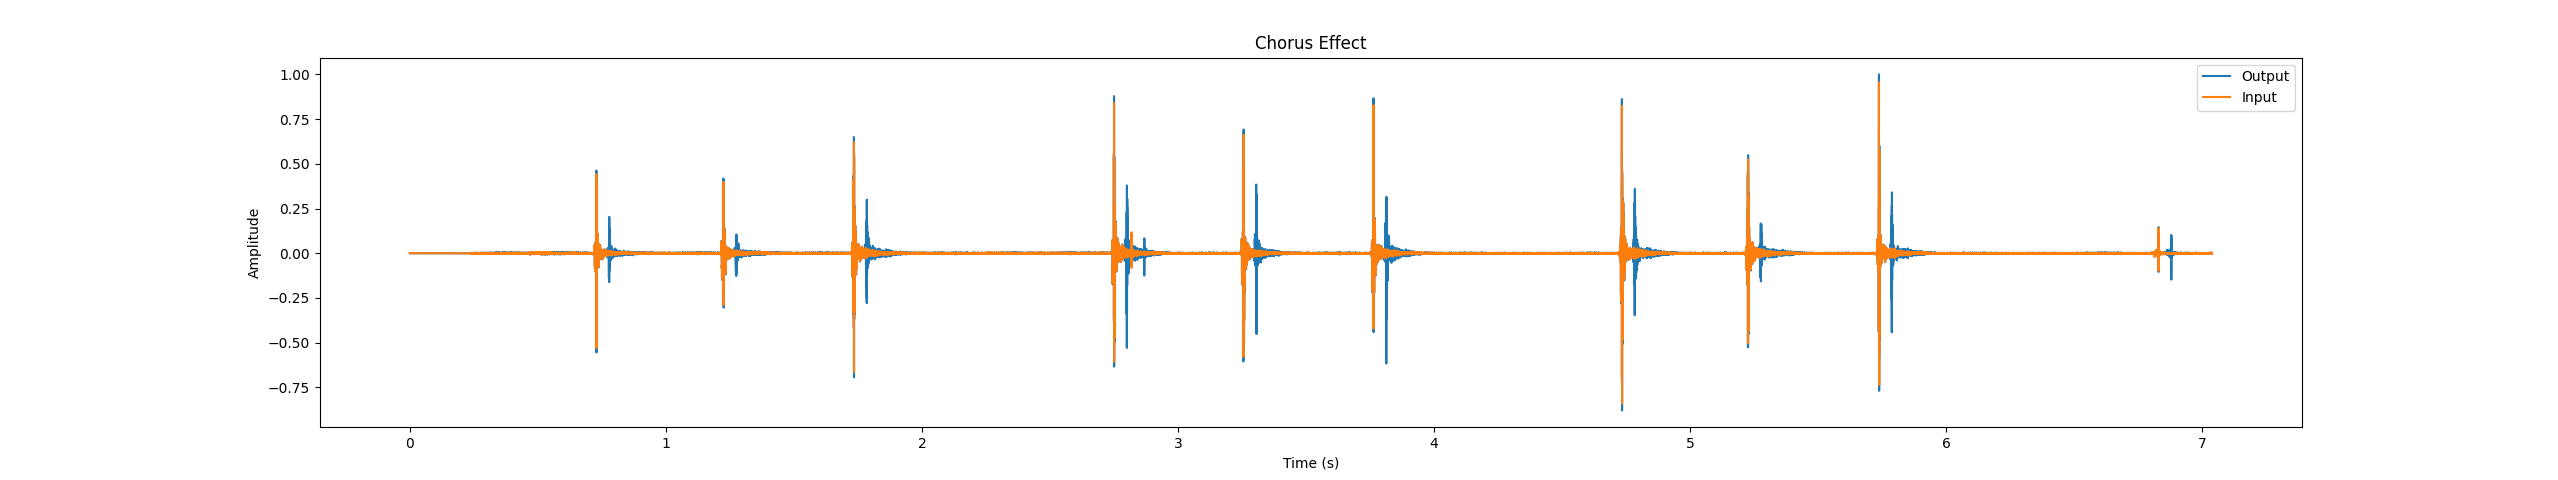
\includegraphics[width=1.75\textwidth]{chorus_finger-snapping.png}}
	\caption{\textit{Chorus}: pucketanje prstima}
	\label{fig}
\end{figure}
\begin{figure}[!htb]
	\centerline{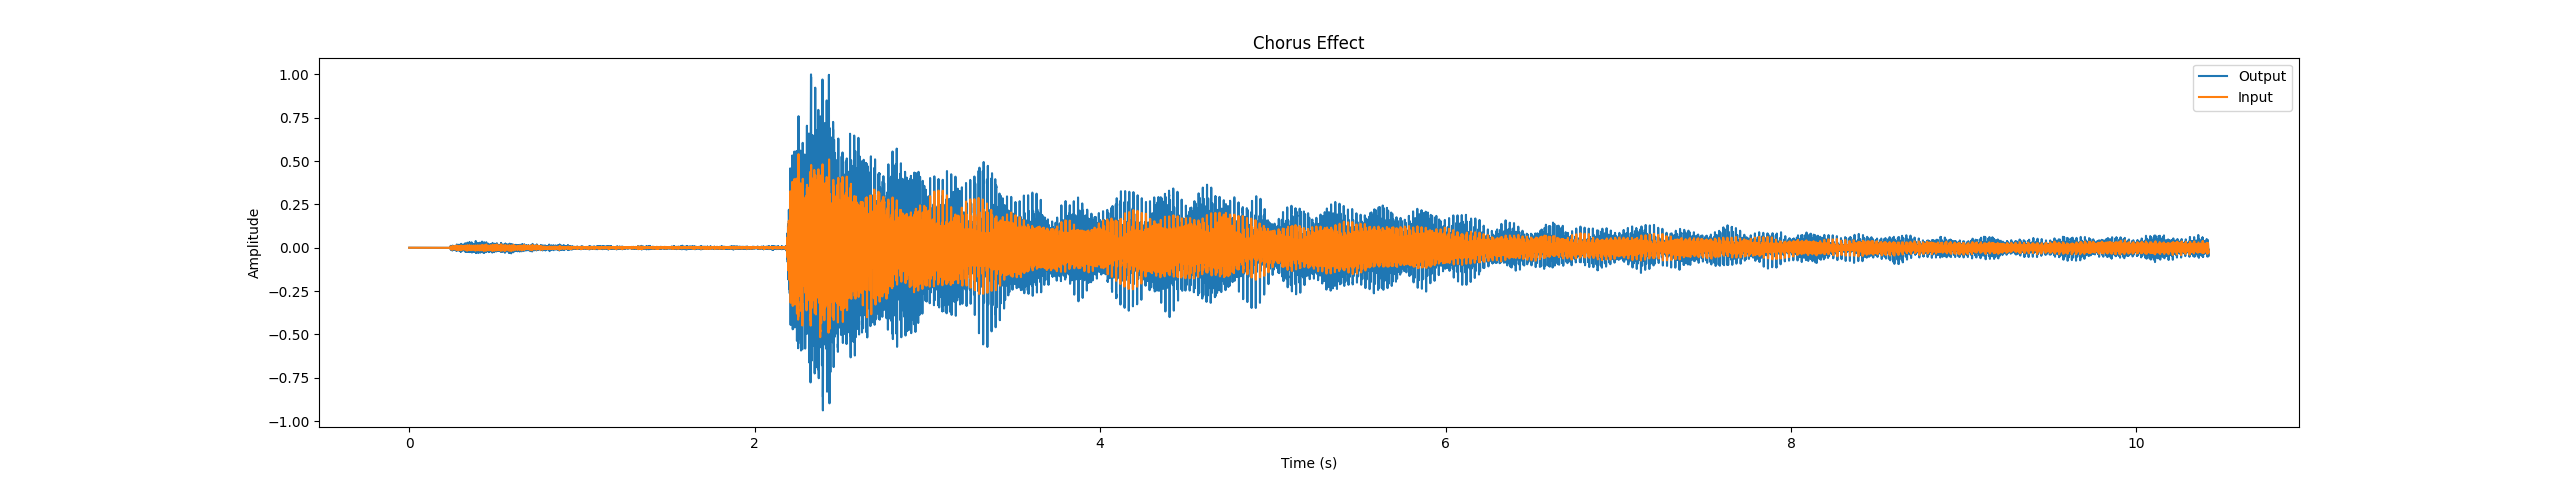
\includegraphics[width=1.75\textwidth]{chorus_strum.png}}
	\caption{\textit{Chorus}: prolaz (eng. \textit{strum}) po žicama gitare}
	\label{fig}
\end{figure}
\begin{figure}[!htb]
	\centerline{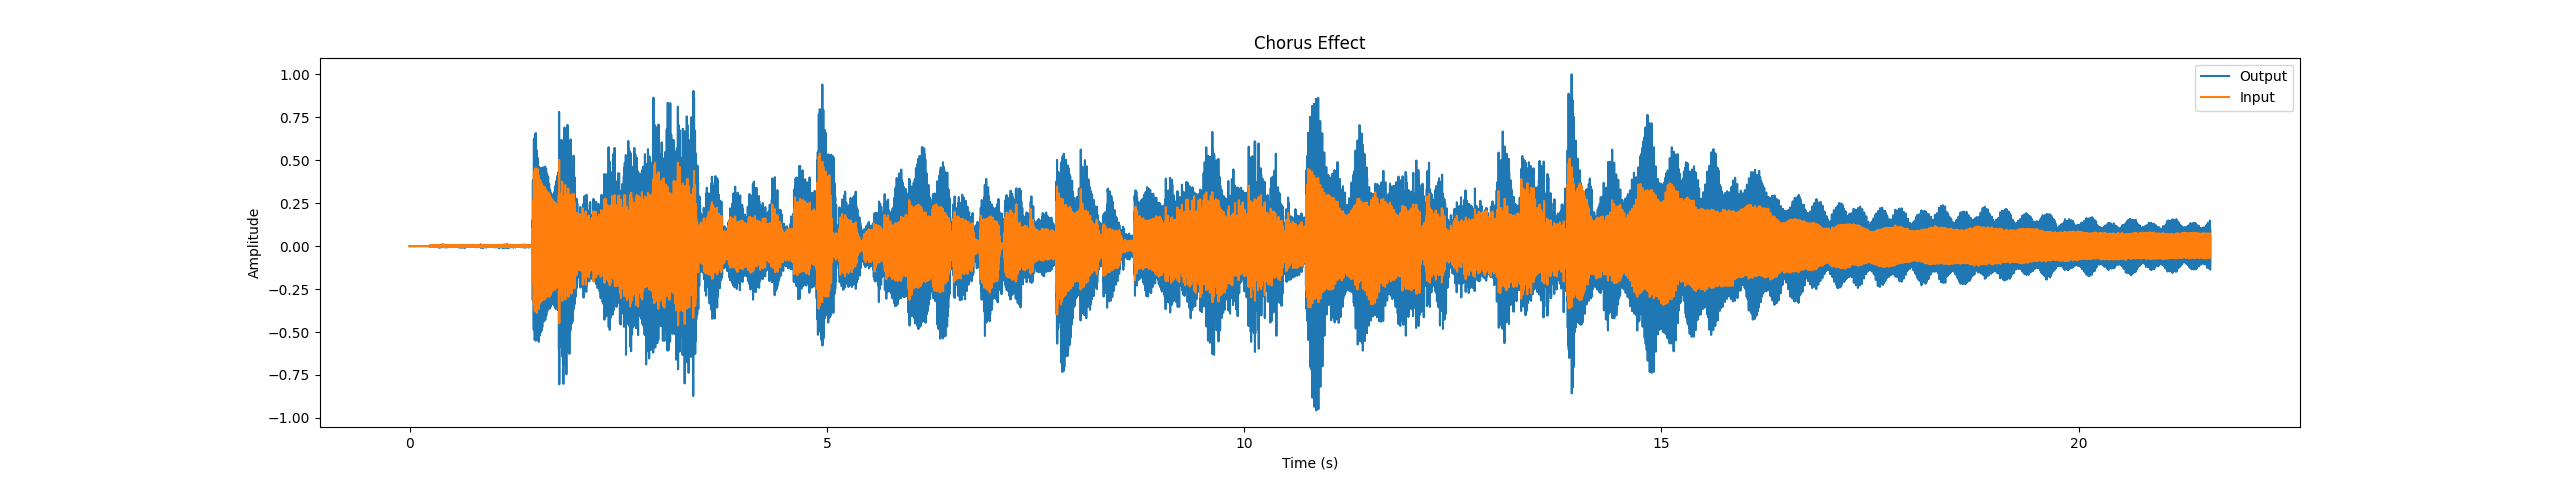
\includegraphics[width=1.75\textwidth]{chorus_rising-sun.png}}
	\caption{\textit{Chorus}: rif (eng. \textit{riff}) pjesme \textit{House of the Rising Sun}}
	\label{fig}
\end{figure}

\chapter{Implementacija u praksi}

\section{Zašto Python?}

U ovom seminaru predstavljeni su primjeri audio efekata i njihove implementacije u programskom jeziku Python. Jedan od glavnih razloga za ovaj izbor je jednostavnost korištenja biblioteke Matplotlib, koja omogućuje stvaranje jasnih i informativnih vizualizacija ulaznih i izlaznih signala u vremenskoj i frekvencijskoj domeni. Ova biblioteka pruža jednostavno i intuitivno sučelje za iscrtavanje i oblikovanje grafikona, što je čini idealnim izborom za demonstracijske i prezentacijske svrhe. Uz to, programski jezik Python ima jednostavnu i lakše čitljivu sintaksu, što ga čini dobrim izborom za demonstracije i dobrom alternativom pseudokoda.

\section{Zašto ne Python?}
Vrijedno je napomenuti da je za zadatke digitalne obrade signal C++ učinkovitija i brža opcija od Pythona. Međutim, u ovom slučaju glavni cilj je brzo implementirati i predstaviti dokaz koncepta određenih audio efekata, stoga je jednostavnost korištenja Matplotlib biblioteke i drugih korisnih biblioteka poput numpy Python učinila boljim izborom. Sposobnost brzog iscrtavanja ulaznih i izlaznih signala na jasan i informativan način presudna je za razumijevanje ponašanja efekata i kako oni utječu na signal.

\newpage
\section{Kod}
\subsection{Delay}
\begin{lstlisting}
	def delay(input_signal, fs, delay_time):
		# Izracun broja zakasnjelih uzoraka preko vremena kasnjenja
		delay_samples = int(fs * delay_time)
		
		# Stvaranje filtra kasnjenja pomakom ulaznog signala za broj zakasnjelih uzoraka
		delay_filter = np.pad(input_signal, (delay_samples, 0), 'constant')
		# Prosirenje ulaznog signala do duljine filtra kasnjenja
		input_signal = np.pad(input_signal, (0, delay_samples), 'constant')
		
		output_signal = input_signal + delay_filter
		
		# Normalizacija izlaznog signala kako bi se sprijecilo odrezivanje
		output_signal /= np.max(np.abs(output_signal))
		
		return output_signal
\end{lstlisting}

\pagebreak
\subsection{Reverb}
\begin{lstlisting}
	def reverb(input_signal, fs, decay_time, delay_time):
		# Stvaranje izlaznog signala kao niza nuli
		output_signal = np.zeros_like(input_signal)
		
		# Izracun faktora slabljenja preko vremena slabljenja
		decay_factor = np.exp(-1 / (fs * decay_time))
		# Izracun broja zakasnjelih uzoraka preko vremena kasnjenja
		delay_samples = int(fs * delay_time)
		
		# Primjena reverb efekta uz dodatan feedback faktor
		feedback_gain = 0.5
		
		for i in range(len(input_signal)):
			# Suma ulaznog sa zakasnjelim i oslabljenim signalom za trenutni uzorak
			if i >= delay_samples:
				output_signal[i] = input_signal[i] + feedback_gain * decay_factor * output_signal[i - delay_samples]
			else:
				output_signal[i] = input_signal[i]
		
		# Normalizacija izlaznog signala kako bi se sprijecilo odrezivanje
		output_signal /= np.max(np.abs(output_signal))
		
		return output_signal
\end{lstlisting}

\pagebreak
\subsection{Chorus}
\begin{lstlisting}
	def chorus(input_signal, fs, depth, rate, delay_time):
		# Stvaranje izlaznog signala kao niza nuli
		output_signal = np.zeros_like(input_signal)
		
		# Izracun broja zakasnjelih uzoraka preko vremena kasnjenja
		delay_samples = int(fs * delay_time)
		# Priprema LFO-a
		lfo_period = int(fs / rate)
		lfo = depth * np.sin(2 * np.pi * np.arange(len(input_signal)) / lfo_period)
		
		# Primjena chorus efekta koristenjem LFO-a i kasnjenja
		for i in range(len(input_signal)):
			# Suma ulaznog sa zakasnjelim i moduliranim signalom za trenutni uzorak
			if i >= delay_samples:
				output_signal[i] = input_signal[i] + lfo[i] * input_signal[i - delay_samples] + (1 - depth) * output_signal[i - delay_samples]
			else:
				output_signal[i] = input_signal[i]
		
		# Normalizacija izlaznog signala kako bi se sprijecilo odrezivanje
		output_signal /= np.max(np.abs(output_signal))
		
		return output_signal
\end{lstlisting}

\chapter{Zaključak}
Seminar je pokrio nekoliko važnih koncepata u digitalnoj obradi signala (DSP) s fokusom na obradu audio signala u stvarnom vremenu. Definirane su osnove DSP-a kao što su kvantizacija i FFT te se raspravljalo o važnosti konvolucije u stvaranju različitih vrsta audio efekata. Zatim su predstavljeni specifični audio efekti kao što su delay, reverb i chorus, i pokazano je kako se ti efekti postižu različitim varijacijama principa kašnjenja. Kroz različite primjere audio signala pokazano je kako ti efekti utječu na ulazni signal. Na kraju su prikazane pojednostavljene implementacije audio efekata u jeziku Python. Dok je Python korišten u ovoj implementaciji zbog svoje jednostavnosti i praktičnosti upotrebe crtanja grafikona, vrijedno je napomenuti da je C++ prikladniji za digitalnu obradu signala zbog brzine svoje izvedbe.

\bibliography{literatura}
\bibliographystyle{fer}

\begin{sazetak}
Ovaj seminar istražuje obradu audio signala u stvarnom vremenu. Pokriva temeljne koncepte digitalne obrade signala i digitalnog zvuka te raspravlja o kompromisu između složenosti obrade, kvalitete i latencije. Isto tako demonstrira kako implementirati različite audio efekte poput kašnjenja (delay-a), reverb-a i chorus-a koristeći programski jezik Python. 
\newline
\kljucnerijeci{audio signali, digitalna obrada signala, obrada u stvarnom vremenu, Python}
\end{sazetak}

\engtitle{Real-time audio signal processing}
\begin{abstract}
This seminar explores real-time audio signal processing. It covers the fundamental concepts of digital signal processing and digital audio, and discusses the trade-offs between processing complexity, quality, and latency. It also demonstrates how to implement various audio effects such as delay, reverb and chorus using the Python programming language.
\newline
\keywords{audio signals, DSP (Digital Signal Processing), real-time processing, Python}
\end{abstract}

\end{document}
